%==================================================================================================
%   LUKES THESIS TEMPLATE 1.2
%   -------------------------
%   This template is based upon the offcial IMM PhD Thesis template, it is enhanced with a number
%   of new features and a number of errors have fixed. This template is intended to be complied to
%   PDF using PDFLATEX and is tested using the MiKTeX 2.9 LaTeX distribution.
%   It is based on the official DTU-IMM Thesis template by Finn Kuno Christensen in 2009.
%   Small bugfixes by Kasper Laursen in 2012 and 2013.
%   -------------------------
%   Last Updated: 2012-09-19
%   Contact: lthhe@imm.dtu.dk
%==================================================================================================
%
%==================================================================================================
% DOCUMENT SETUP
%==================================================================================================
\documentclass[10pt,twoside]{book}                  %Official DTU-IMM Thesis document setup
%
%Set to 'print' for printed version, use 'net' for online version
\def\thesisversion{print} 
%
%==================================================================================================
% PACKAGES
%==================================================================================================
\usepackage{LukeThesis}                             %Import Thesis base style
%input{PhDMacros}                                   %Thesis specific macros
%
%==================================================================================================
% THESIS PROPERTIES (Modifiy these fields with your details)
%==================================================================================================
\def\thesisauthor{Luke Herbert}                     %Author
\def\thesistitle{Something something}               %Title
\def\thesishandin{01-January}                       %Submission date (Day-Month}
\def\thesisdegree{PhD}                              %Degree ('B.Eng', 'B.Sc.', 'M.Sc.' or 'PhD')
\def\thesisyear{2013}                               %Submission year
\def\thesisnumber{????}                             %DTU-IMM Serial number (do not include year)
\def\thesisISSN{0000-0000}                          %ISSN number
\def\thesiskeywords{Keywords are, comma separated}  %PDF keywords
\derivethesisprops                                  %Derive dependent properties
%
%==================================================================================================
% SECTION NUMBERING SETUP
%==================================================================================================
\setcounter{tocdepth}{2}                            %2 adds sections up to subsections
\setcounter{secnumdepth}{3}                         %Subsubsections get a number when this is 3
%
%==================================================================================================
% THESIS STRUCTURE  (Modifiy to include more chapters etc)
%==================================================================================================
\begin{document}
%------------------------
%Pre-frontmatter material
%------------------------
\prefrontmatter  
%--------------------
%Frontmatter material
%--------------------
\frontmatter
\pagenumbering{roman}                               %Set frontmatter numbering style
\chapter{Summary - English}

The understanding of human mobility patterns constitutes a focus point in the
science world today and has been the main topic of numerous studies. The data
that has been used in order to analyze the mobility patterns varies from GPS
data, to data collected by telecommunication towers and even to information
extracted from the dispersion of bank notes. In this paper we study the
inferring of mobility patterns from Wifi data. We analyze methods that can be
used for identifying stop locations with the help of Wifi data, we compare our
results with stop locations identified using GPS data and we explore the degree
of predictability of human travel trajectories.

% The understanding of human mobility patterns constitutes a focus point in the
% science world today and has been the main topic of numerous studies. The data
% that has been used in order to analyze the mobility patterns varies from GPS
% data, to data collected by telecommunication towers and even to information
% extracted from the dispersion of bank notes. In this paper we study the
% inferring of mobility patterns from Wifi data. We analyze methods that can be
% used for identifying stop locations with the help of Wifi data, we compare our
% results with stop locations identified using GPS data and we explore the
% degree of predictability of human travel trajectories.
                                   %English summary of Thesis
\markboth{}{}                                       %Set headings (left)(right)
%\chapter{Summary - Danish}

Forståelsen af menneskers bevægelsesmønstre er et aktivt forskningsfelt og
omdrejningspunkt for talrige studier. Datamaterialet bag disse analyser spænder
bredt, fra GPS-data til data indsamlet via telekommunikationsmaster, og helt til
bevægelsesmønstre udledt på baggrund af diffusion af pengesedler. I denne
afhandling ser vi nærmere på hvordan bevægelsesmønstre kan udledes fra WiFi
data. Vi analyserer metoder, som på baggrund WiFi data, kan bruges til at
identificere "stop locations" -- steder hvor en person opholder sig i længere
tid -- og sammenholder disse resultater med "stop locations" identificeret ved
hjælp af GPS data. Endelig undersøger vi i hvilken grad menneskers
bevægelsesmønstre kan forudsiges.
                                   %Danish summary of Thesis
\markboth{}{}                                       %Set headings (left)(right)
\chapter{Preface}

This thesis was prepared at the Department of Applied Mathematics and Computer
Science at the Technical University of Denmark in fulfilment of the requirements
for acquiring an M.Sc. in Computer Science and Engineering.

The thesis describes the steps taken in order to explore methods which can be
used in order to determine stop locations as well as the predictability of human
mobility based on Wifi data.

%==================================================================================================
% SIGNATURE AREA
%==================================================================================================
\vspace{20mm}
\begin{center}
    \hspace{20mm} Lyngby, \thesishandin-\thesisyear
    \vspace{5mm}
    \newline
  %Update signature image file in line below
    
\includegraphics[scale=0.5]{figures/SignatureDummy.jpg}
\end{center}
\begin{flushright}
    \thesisauthor
\end{flushright}
% % % EOF % % %                                     %Preface
\markboth{}{}                                       %Set headings (left)(right)
\chapter{Acknowledgements}

I would like to thank my supervisors, Sune Lehmann and Jakob Eg Larsen for their
guidance and feedback throughout the work done for this thesis.

I would also like to thank Andrea Cuttone, Piotr Sapieżyński, and David Kofoed
Wind for their advice and assistance with technical issues.

Finally, I would like to thank my family and friends for their constant support
and encouragements.

                            %Acknowledgements
\markboth{}{}                                       %Set headings (left)(right)
%------------------
% Table of contents
%------------------
\newpage\mbox{}\newpage
\chaptermark{Contents}
\pdfbookmark{\contentsname}{toc}
\renewcommand{\sectionmark}[1]{\markright{#1}}
\sectionmark{Contents}
\addtolength{\parskip}{-\baselineskip}
\tableofcontents
\addtolength{\parskip}{\baselineskip}
\renewcommand{\sectionmark}[1]{\markright{\thesection\ #1}}
%-------------
% Main content
%-------------
\mainmatter
\chapter{Introduction}

The United Nations (UN) Department of Economic and Social Affairs' Population
Division is in charge of preparing once every two years an estimation of what we
are to expect the growth rate for the world population to be in the following
years. Occasionally, world population projections over a longer period of time
are created as well. In $2004$, the UN has made predictions about the trends in
population growth up until $2300$ \cite{UNWp}. The predictions show that the
population will increase to reach a peak of $9.22$ billion by the time of $2075$
and then it will decrease slowly to $8.97$ billion by $2300$. These estimations
bring up different aspects regarding our quality of life which is a topic that
will only increase in importance with the population growth. For example, we
need to think about more efficient ways in which we can develop the urban
regions or our transportation infrastructure in order to ensure that space is
used in a responsible and optimal manner. Also, it is important to understand
how epidemics spread and how they can be contained in order to avoid devastating
pandemics from tacking place.

The rapid evolution of technology has equipped us with tools that can be used in
order to gather large amounts of information about human behaviour and mobility
patterns. This information can be employed by scientists in research and study
programs in order to obtain facts and results that can be used to solve possible
problems which are sure to appear due to the rise in population that seems to be
facing us. Current studies about the predictability of human mobility uncovered
remarkable findings which suggest that we might be less spontaneous when it
comes to choosing our destinations than we might think we are. These results can
prove to be of tremendous help in the making of decisions about transportation
infrastructure and they can even give us an insight on how diseases are
spreading from region to region.

Due to the importance of the results that can emerge from studying the
predictability of human mobility, we have conducted a study that is focused on
this topic, mainly the inferring of mobility patterns from Wifi data. In order
to understand what defines a location we analyze different methods that can be
used for extracting stop locations from the gathered Wifi data. We discuss and
propose a solution for determining if two identified locations represent in fact
the same geographical stop location. This helps us construct a long term image
of the travel trajectories associated to the users who are providing the data.
We compare the results we have, our stop locations obtained from the Wifi data,
to results generated using GPS data and we explore the degree of predictability
of human travel trajectories based on the image we are able to create about the
mobility patterns over a longer period of time.

The detailed explanation of all steps made during our work, as well as the
results and observations we have come across are structured into eight different
chapters. Chapter $2$ (Related work) presents previous findings and studies
conducted on the topic. Chapter $3$ (Prerequisites and tools) presents the
elements that have contributed to making this work possible: data gathered with
the help of volunteers, implementation, visualization and data analysis tools
etc. Chapter $4$ (Data processing) presents the data that has been used during
our work as well as the way in which we have eliminated interferences and noise
from the received data. Chapter $5$ (Extracting locations from Wifi data)
presents all the steps that have been taken from the data analysis up to the
analysis of the different algorithms that we have experimented with in order to
extract the locations from the Wifi data. Chapter $6$ (Location matching)
presents the techniques we have considered in order to estimate if two given
locations that have been discovered by using a location extraction algorithm can
be catalogued as being the same location based on defining characteristics.
Chapter $7$ (Entropy and predictability) presents the calculations made in order
to determine the different entropy values and predictability that can be
attributed to the users based on the location information that emerged from
their data as well as what these values represent. Chapter $8$ (An evaluation
of Wifi positioning accuracy) presents the comparison made between the results
we have obtained from the Wifi data and the stop locations which can be
extracted from the analogue GPS data. Chapter $9$ (Discussion and future work)
presents a summary of the results and observations which have emerged during
our work as well as proposed topics and directions for further work on the
present subject.
                                  %Chapter 1
%\chapter{Related work}
% 7 pages
There is a high interest and a huge amount of work the scientific community
dedicates to understanding the patterns of human mobility. The knowledge we
can gain from the results of this work has the potential to benefit a wide
variety of industries from the modeling and maintenance of the transportation infrastructe,
to the medical industry where we can use this knowledge in trying to prevent the
spreading of epidemies. \ref{Brockmann08} %TODO - add references

Various studies have been conducted in order to gain a better understanding of
the human mobility patters. These studies give us results that seem to support
each other in the idea that people are less spontaneous than they would like to
think themselves and that, indeed, our behaviour shows that we are quite rooted
into habbits when it comes to the way we travel.

\section{Mobility patters uncovered by the disipation on bank notes}
Brockmann, Hufnagel and Geisel\ref{Brockmann06} have
analyzed the human movement based on the way bank notes were dispersed through
the United States (excluding Alaska and Hawaii). Their study shows that a
relatively small percentage of bank notes ($23.6\%$) traveled for more than
$800$ km, while a fraction of $19.1\%$ did not traveled for more than $50$ km
even after a year of being observed. The possible explanation the authors have
given for these findins are that, in general, people would be less inclined to
leave the areas of the large cities or the places they usually conduct their
lives.

The problem identified with this approach for tracking individuals is that the
bank notes exachange hands and the behaviour which is identified by the way they
circulate can't be attributed to a single individual, but rather to different
ones that at any moment have had the bank note in their posession. Despite this,
the result have a high scientific value as they do identify patterns in human
travel behaviours in general.

\section{Mobility patterns of mobile phone users}
A. L. Barabasi, M. C. Gonzalez and C. A. Hidalgo have conducted a study
\ref{Barabasi08} that deals with studying the trajectories of over $100000$
mobile phone users with anonymized identities. The study was conducted in order
to see if there are any patterns in our mobility habbits. Among the things that
have been subjected to testing was the return probability of individuals in the
same place as in the past. The study shows there is, in general, a peak in the
return probability after $24$, $48$ or $72$ since they have left a particular
location. This shows that we humans tend to visit locations periodically. This
can be explaineQd by our going to places such as work, school, grocery shops
near our home etc.

The authors have also ranked the locations the mobile phone users frequented
based on the number of times they have been spotted nearby. The results for this
have shown that the probability of finding someone near a location that is
ranked for them with a level $L$ can be estimated with $1/L$. Another
interesting finding that is mentioned in the paper is that, in general, people
seem to be spending the majority of their time in just a few locations, while
diving the remaining time just between a limited number of locations that varies
for the subjects from as low as $5$ to around $50$.

There are some note worthy plots that the authors present in the paper. They can
be seen in figure{} and they show that most people travel over short distances,
yet there is a small number of people that regularly travel over big distances.

The results of this study are a major indicator that individuals display a high
level of regularity and that we have a tendency to spend most of our times in
places that are familiar to us, or that require us to visit them regularly
(e.g. home, work).

\section{Mobility patterns in massive multiplayer online games}
R. Sinatra and M. Szell have studied the way in which users of a massive
multiplayer online game behave inside the virtuale universe provided by the
mentioned game \ref{Sinatra14}. It has been established that the massive
multiplayer games provide people with a virtual reality where they can interact
with others through their characters and can, in fact, form groups and, as
such, display both individual as well as collective behaviour actions that can
translate to the non-virtual world \ref{Ball03}.

This study gives an interesting insight into the habbits and actions of the
characters which are controlled by the players. Among the things the authors
have analyzed are the predictability of the characters, the entropy generated
by the mobility of the characters in the virtual universe and general
strategies or patterns that could be observed.

The game the authors have been using for the study is called
Pardus \ref{Pardus}. This game is quite complexe, as it allows the manifestation
of normal real-life activities such as the creation of alliances or friendships,
communication between the players, economic related action, or even actions
which have a negative conotation such as attack of another user, removal of a
friendship link etc. The universe of the game consists in hundrets of nodes
which represent cities or sectors in the game. These virtual cities are tied to
each other through links which mark the posibility for the users to move their
characters from one place to another.

By analyzing the why in which characters have interacted through the years, the
authors have observed that the mobility of the characters through the univers is
highly predictable, as users in general will seem to be chosing a random
location to visit next in just about $10\%$ of the cases.

\section{Eigenbehaviours}
N. Eagle and A. S. Pentland analyze data of individulas and communities with the
purpose of trying to predict and cluster the daily habbits and behaviour of
people \ref{Eagle09}. The consider that the behaviour of one person throughout a day
can be close to a sum of their primary eigenbahaviours throughout that day. The results
of the study have shown that when having a weighted sum calculated for the first
half of a day, the behaviour of the same person throughout the remaining of the
day can actully be approximated with $79\%$ accuracy. 

The results have applicability in more fields, as they allow us to consider the
possibility of clustering people into various communities based on the
similarity of their behaviours. It goes even further, as the findings show that
this enables the possibility of calculating similarity for groups as well and
thus permiting the a classification that, according to the experiment, can be
$96\%$ accurate for determining affiliations in the social network of a
particular population.

As a last observation in the paper by N. Eagle and A. S. Pentland it is stated
that eigenbehaviours can be used in order to identify the possible friendship
ties between people. The observations in this paper have been done based on the
Reality Mining dataset that tracked the behavior for 100 individuals at MIT for
the duration of one year.

\section{Human movement recorded through real traces}
Studies as the ones with the travel of bank notes or the recorded location of
mobile users through telephone is not very exact and does not reflect the real
traces for the people. They do provide a very useful estimation, however with
the technology that we have access to nowadays, we are able to record mobile
phone users' real traces either through GPS or WiFi. The data that can be
acquired through these means allows us to conduct studies that can take into
consideration a very good approximation of the real location of individuals.

In the paper by M. Kim, D. Kotz and S. Kim \ref{Kim06}, the authors present us
with a method in which the locations of users can be estimated based on the WiFi
signals that their devices register. The experiment is conducted cosndiering the
data for a duration of $13$ months. The user traces that have been used consist
of the trace data from the Darmouth College. The mobility traces are defined as
the lists of access points that are associated to a user's devices at a given
timestamp. 

The mobility traces allowed the authors to extract the tracks (locations) of the
users. They have explored three methods in which the location can be extracted
from the data. The first approach presumed the calculation of the center
(intersection of medians) of the traingled defined by the past three access
point associations of the mobile device of the user. This approach has a
downside since the devices do not necessarly change the associations in a
periodic manner. This lead to the second approach which consisted in considering
a time window after which the associations needed to be updated in case new
associations have appeared during that time. The thrid and last approach
explored the use of Kalman
filters \ref{KalmanFilter}.

The validation the path extarctors the authors have compared the results with
GPS data. This validation has proven that the type of the used device has at the
moment a significant importance in how acqurate the results can be as it seems
that some devices can be more aggressive in updating the associations with
access points while others try to stay associated with the same access points as
long as possible before switching to new ones. This leads to problems as
different distances between users and access points considered by different
devices and as such it affects the estimated paths. The best estimations have
been given in this experiment by the approach that used the Kalman filters,
however both the other two appraoches have provided fairly good estimations as
well.

Another paper which explores the travel patterns from real data is the one
written by T. S. Azevedo, R. L. Bezerra, C. A. V. Campos and L. F. M. de Moraes
\ref{Azevedo09}. The authors propose another approach for analyzing the mobility
of people. They take into consideration the following movement components:
velocity, acceleration, direction angle change and the pause time and they are
using the GPS data in order to estimate the locations of individuals. The
experiment takes place in a park in Rio de Janeiro and is done based on the
data received from around $120$ volunteers. The results have shown that people
seem to have in general smooth trajectories without abrut changes.
% TODO - social network theory
% TODO - radio landscape obs - Perez Penichet paper
%TODO - Levi flight and people vs animals

% TODO - locations and identifying locations paragraph
% TODO - 2-3 papers on identifying locations
% TODO - paragraph about predictability and entropies (Lu13 - approaching the
% limits of predictability) TODO - 2 papers on this
\section{Entropy and predictability}
One step further from understanding the way we travel from place to place is to
predict our future locations based on a previous knowledge our our past
patterns. There has been an extensive study done in this area of the scientific
playground as well and the results which have emerged up until now are
remarcable.

In the paper by C. Song, Z. Qu, N. Blumm and A. L. Barabasi \ref{Barabasi10},
the authors take up the challenge of studying how predictable people can be.
They analyze the mobility patterns of mobile phone users and calculate the
entropy of these users. The locations are defined by the telephone towers the
users are encountering at hourly intervals and the trajectory of the user is
given by the ordered sequence of these towers. The real entropy of each user i
is calculated as $\Sigma _{T'_{i}\subset T_{i}} P(T'_{i})log_{2}(P(T'_{i}))$,
where $P(T'_{i})$ represents the probability of encountering a time-ordered
subsequence $T'_{i}$ in the sequence of hourly encountered telephone towers
$T_{i}$.

The results for this particular study show that, for the considered users, the
uncertainty of where they could be at a certain moment, based on the real
entropy calculated for them would be very low as they would most probably be in
one of two locations.
%The results show that, for most of the users that were part of this particular
%study, the entropy S has been calculated to be around $0.8$. This means that
%% the real uncertainty when it comes to estimating where a user can be at a
% certain
%moment is $2^{0.8}$ which means $1.74$, so less than $2$ locations.

The authors also take a look into the maximum predictability which can be
expected for a user. Their results show that, with the right algorithm, a user's
future location can be predicted with between $80-93\%$ accuracy. This shows
that we are less sponatenous than we might think and that our mobility patterns
are, in most cases, rooted into a very well established routine.

There have been numerous other methods or experiments conducted in order to
analyze or to forcast human mobility patterns. Some of these methods include the
Markov chain models \ref{Ross09} \ref{Liu96}, the neural networks \ref{Liou03}
or the Bayesian networks \ref{Akoush07} as well as some that work with finite
automaton \ref{Petzold04}. Most of the studies support the idea that people's
actions and travel behavior is indeed far from being random and thus the science
world needs to dedicate further effort and time in order to use this knowledge
in order to improve our quality of life and the world we live in.
                                 %Chapter 2
\appendix
\chapter{Appendix}

\section{Variations for signal strength visualization over time}
\label{appendix_signal_strength}

This section contains various visualizations for different users' scanned access
points over time. On the x axis we have the time frame, while on the y axis we
have the signal strength for the identified access points. The legend presents
only the top $10$ predominant access points (which have appeared the most
during scans), however the plot displays all access points. The figures are
Fig.~\ref{user_6_cross_1d}, Fig.\ref{user_6_star_1d},
Fig.~\ref{user_6_cross_line_1d}, Fig.\ref{user_6_o_line_1d}.

\begin{figure}[!h]
\centering
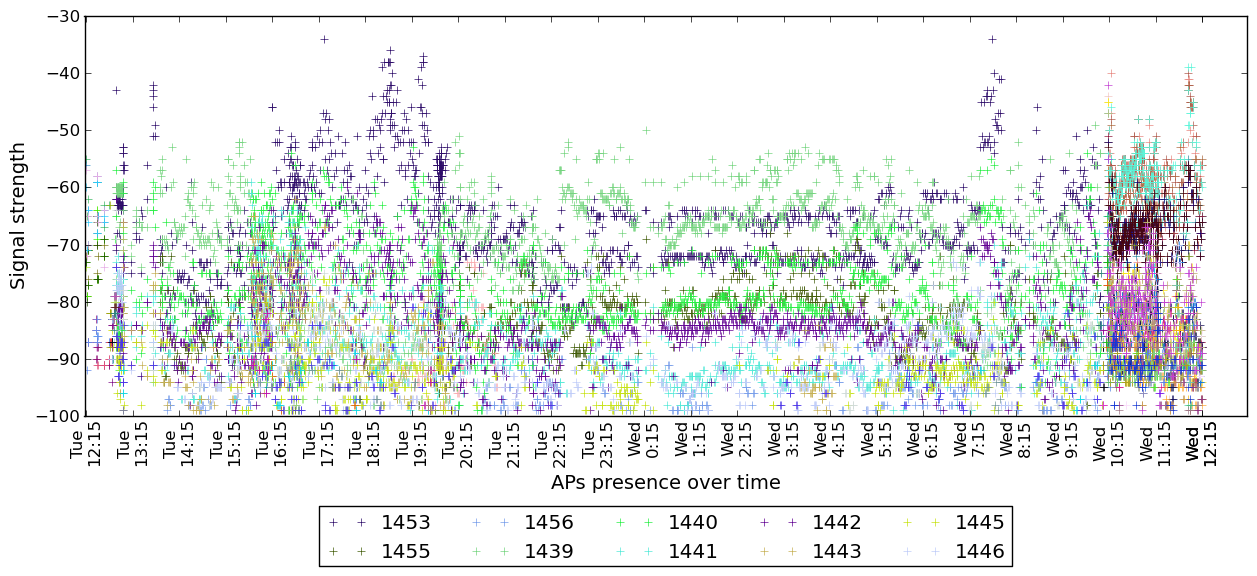
\includegraphics[height =
0.45\textwidth]{figures/cros_user_6_sorted_1days_plot.png}
\caption{Example of the APs registered for userX throughout one day with
``+'' markers}
\label{user_6_cross_1d}
\end{figure}

\begin{figure}[!h]
\centering
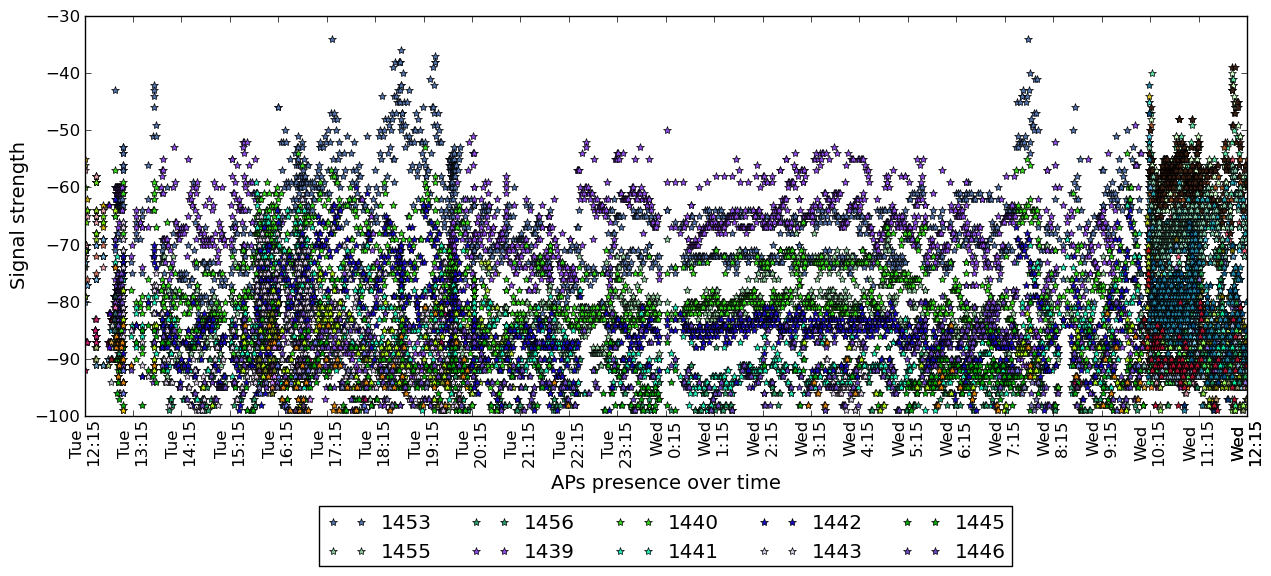
\includegraphics[height =
0.45\textwidth]{figures/star_user_6_sorted_1days_plot.png}
\caption{Example of the APs registered for userX throughout one day with
``*'' markers}
\label{user_6_star_1d}
\end{figure}

\begin{figure}[!h]
\centering
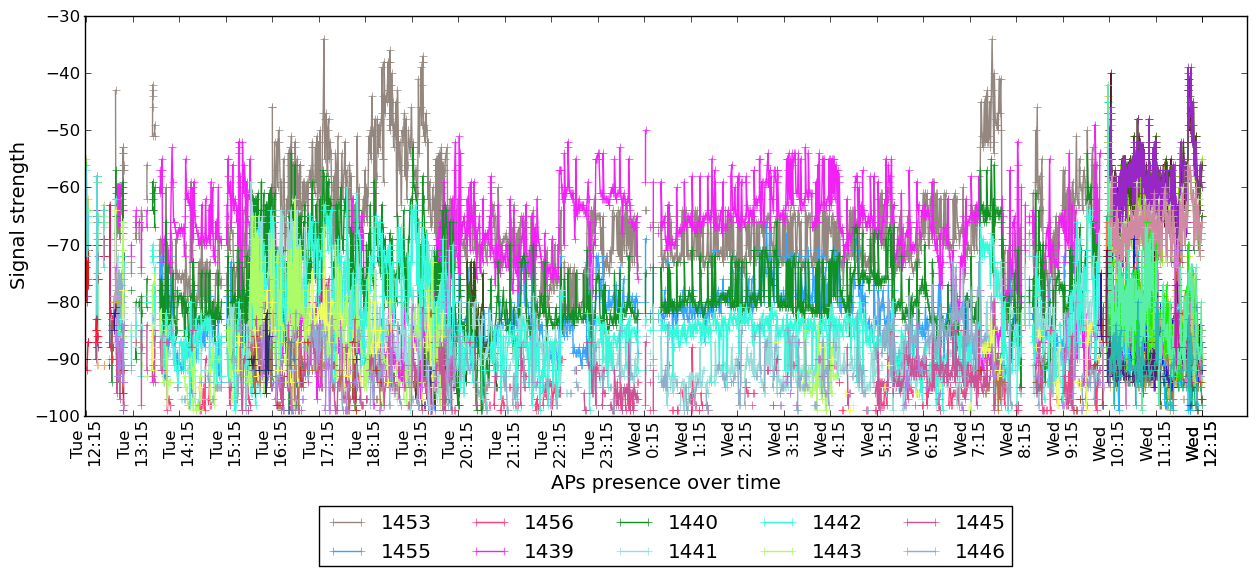
\includegraphics[height =
0.45\textwidth]{figures/cros_line_user_6_sorted_1days_plot.png}
\caption{Example of the APs registered for userX throughout one day with
``+'' and line markers}
\label{user_6_cross_line_1d}
\end{figure}

\begin{figure}[!h]
\centering
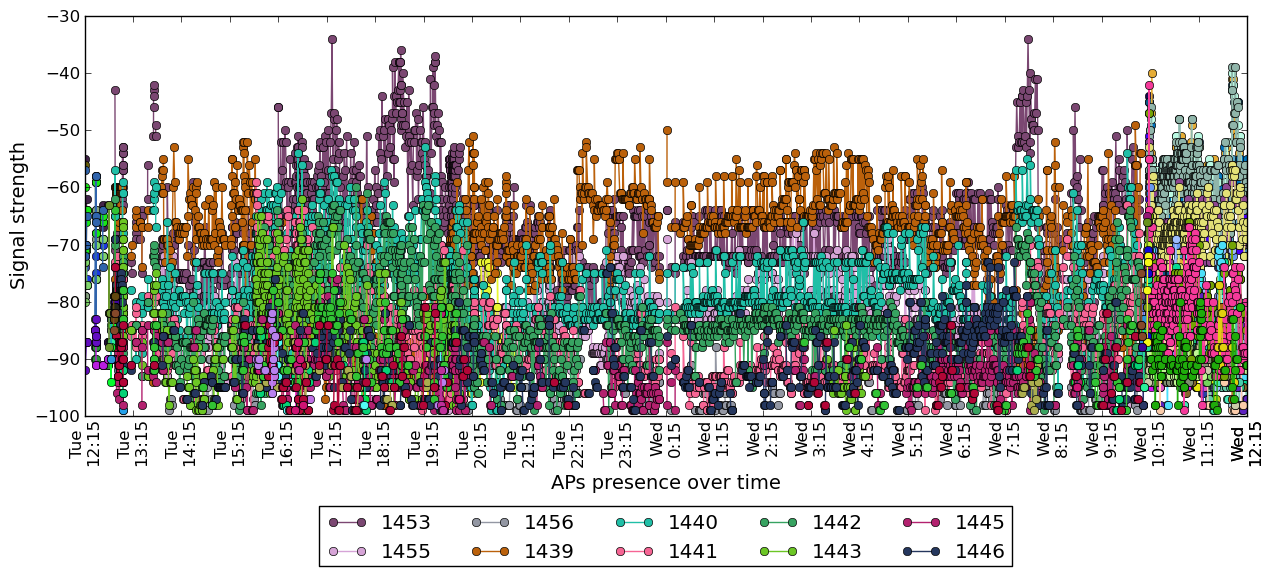
\includegraphics[height =
0.45\textwidth]{figures/o_line_user_6_sorted_1days_plot.png}
\caption{Example of the APs registered for an user throughout one day with
``o'' and line markers}
\label{user_6_o_line_1d}
\end{figure}

\section{Sample density for APs identified for a user}
\label{appendix_sample_density}

This section contains the visualization for the signal strength of different APs
that have been identified as being associated to a user throughout a period of
$1$ day (Fig.~\ref{rssi_6_2nd_day_A}) as well as the sample density
visualizations for the top various APs that were scanned throughout this time
(Fig.~\ref{samples_6_2nd_day_1_A},Fig.~\ref{samples_6_2nd_day_2_A},Fig.~\ref{samples_6_2nd_day_3_A}).

\begin{figure}[!h]
\centering
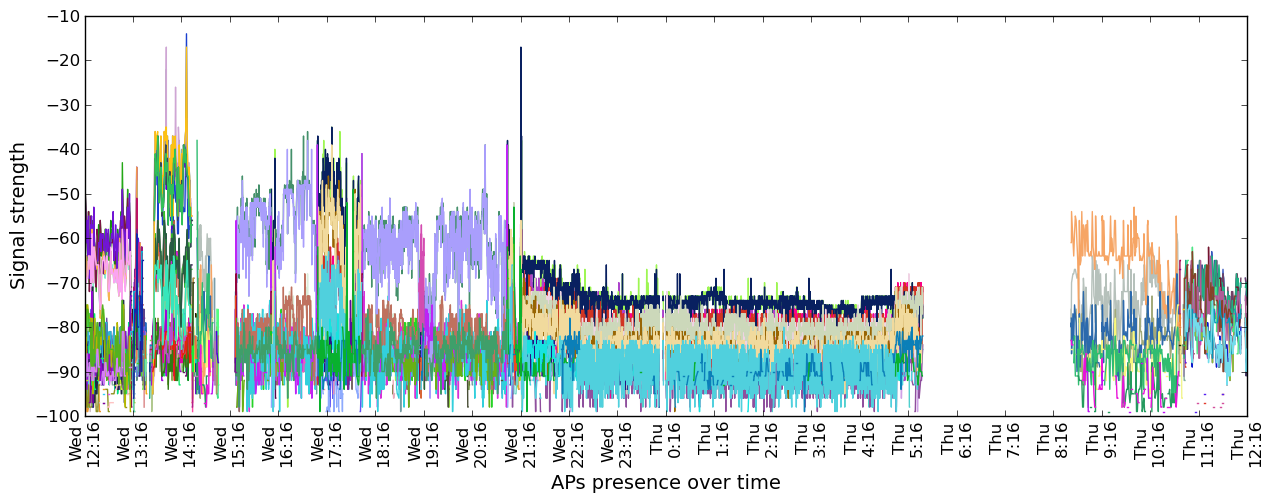
\includegraphics[width =\textwidth]{figures/combinations/user_6_sorted_1days_plot_croped.png}
\caption{Example of the APs registered for userX throughout day 2}
\label{rssi_6_2nd_day_A}
\end{figure}

\begin{figure}[!h]
\centering
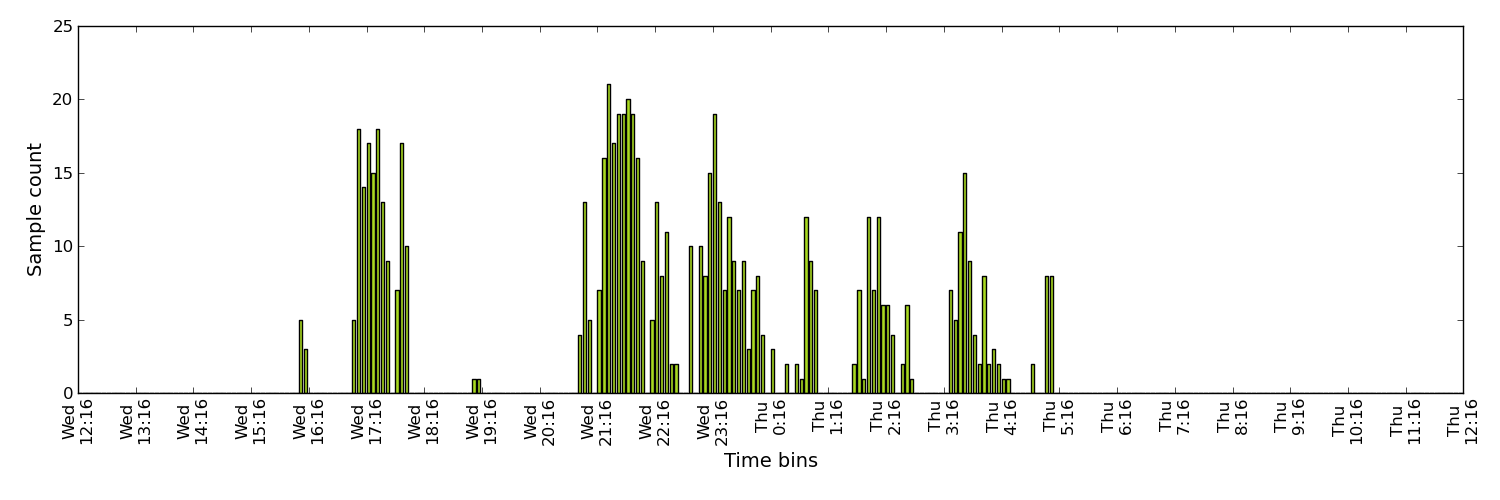
\includegraphics[width =\textwidth]{figures/combinations/ap_15188_histo.png}
\caption{Sample density of AP 15188 for userX}
\label{samples_6_2nd_day_1_A}
\end{figure}

\begin{figure}[!h]
\centering
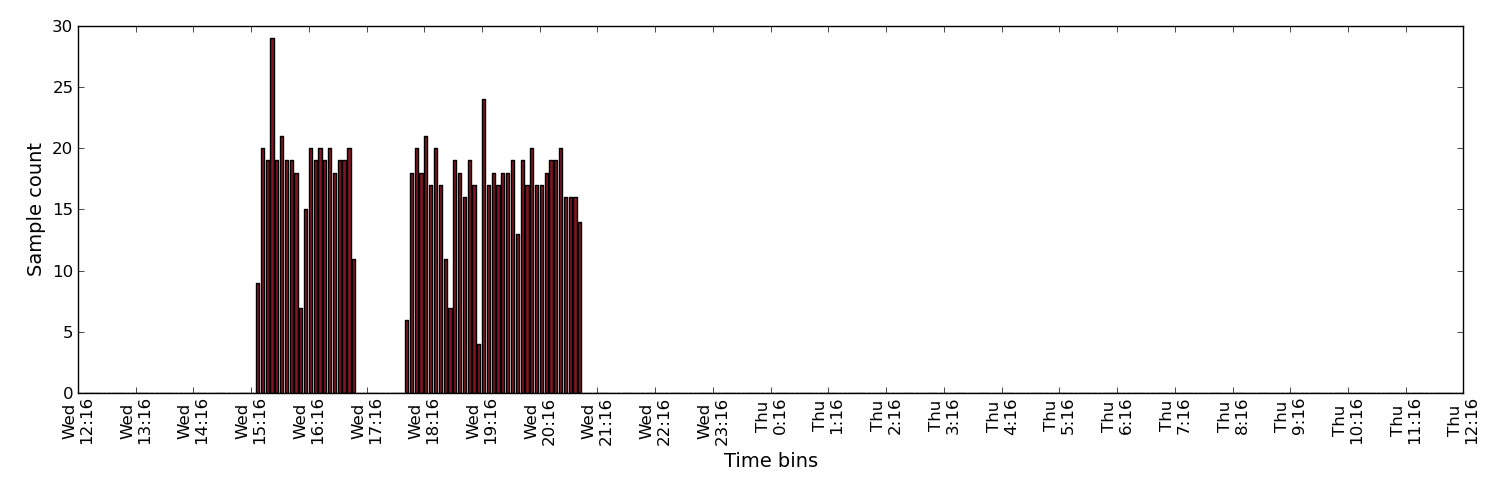
\includegraphics[width =\textwidth]{figures/combinations/ap_15190_histo.png}
\caption{Sample density of AP 15190 for userX}
\label{samples_6_2nd_day_2_A}
\end{figure}

\begin{figure}[!h]
\centering
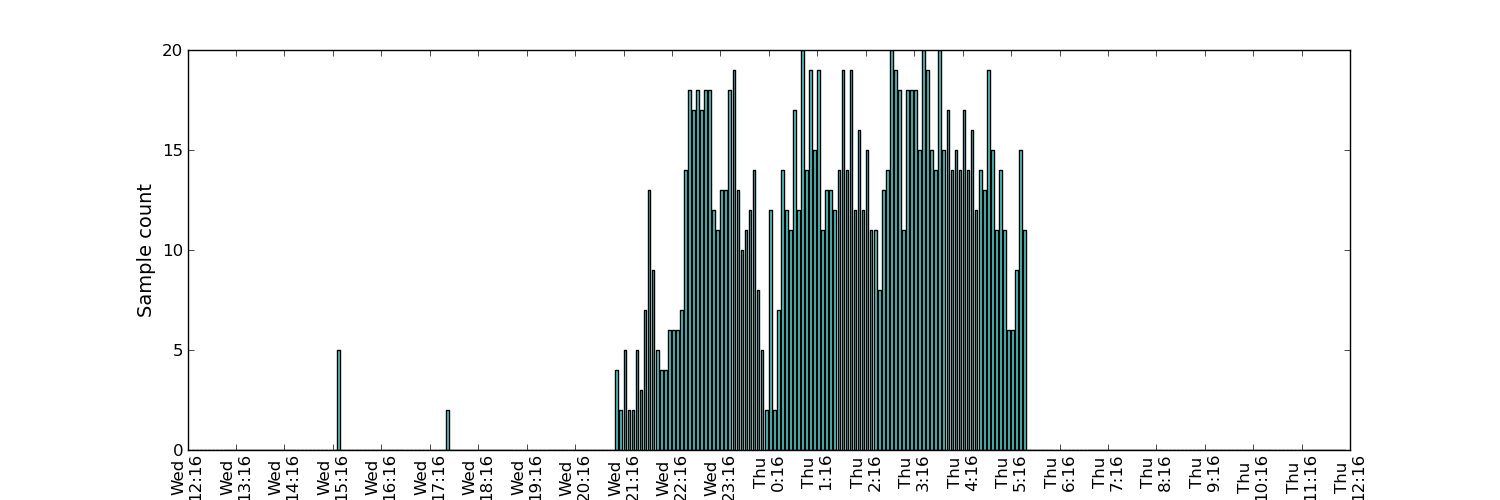
\includegraphics[width =\textwidth]{figures/combinations/ap_3144_histo.png}
\caption{Sample density of AP 3144 for userX}
\label{samples_6_2nd_day_3_A}
\end{figure}

\subsection{Average signal strength for APs identified for a user}
\label{appendix_avg_signal}

This section contains the visualization for the signal strength of APs 15188
(Fig.~\ref{avg_6_2nd_day_1_A}), 15190 (Fig.~\ref{avg_6_2nd_day_2_A}) and 3144
(Fig.~\ref{avg_6_2nd_day_3_A}) calculated for $5$ minutes time bins over the
course of one day from the data gathered for userZ.

\begin{figure}[!h]
\centering
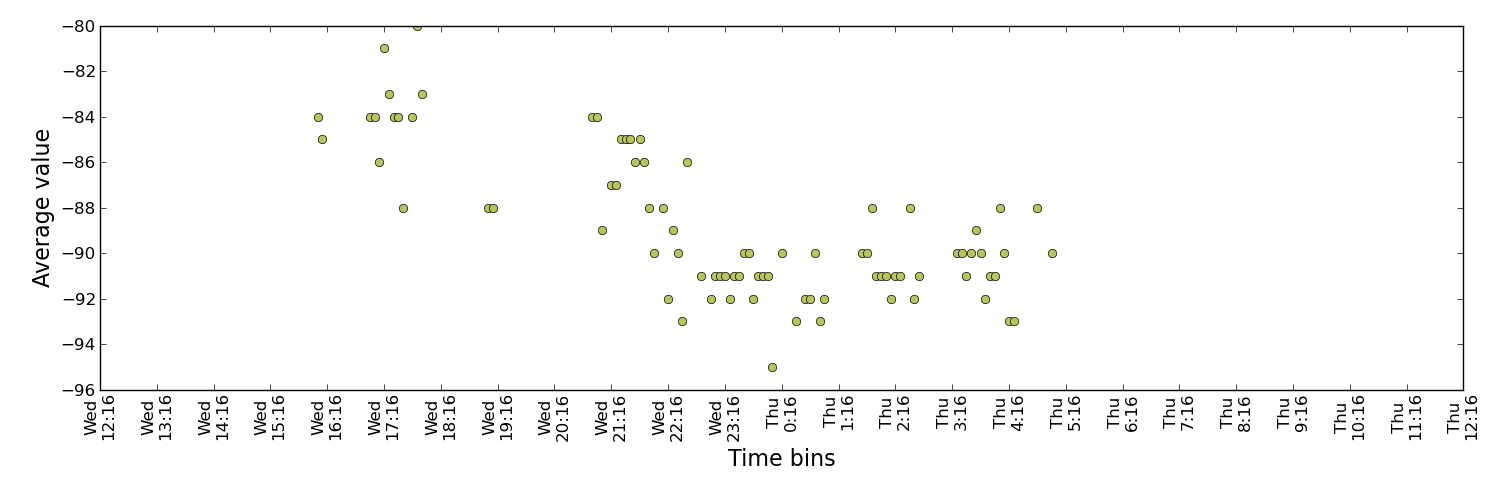
\includegraphics[width =\textwidth]{figures/combinations/user_6_sorted_1days_plot_15188_avg_sig.png}
\caption{Sample density of AP 15188 for userZ}
\label{avg_6_2nd_day_1_A}
\end{figure}

\begin{figure}[!h]
\centering
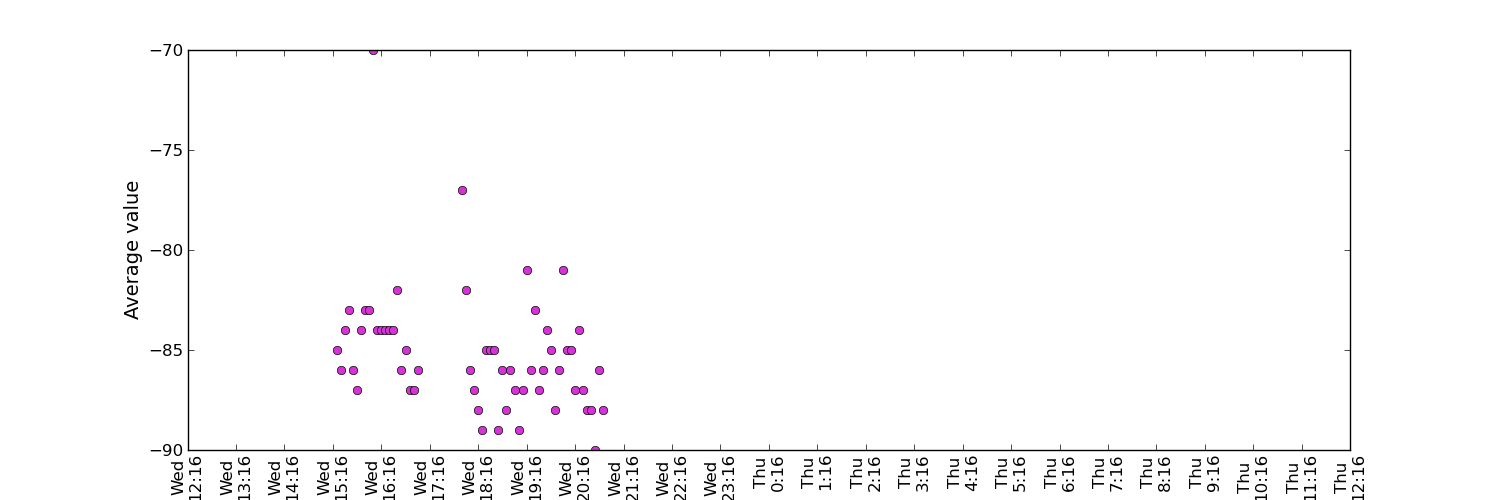
\includegraphics[width =\textwidth]{figures/combinations/user_6_sorted_1days_plot_15190_avg_sig.png}
\caption{Sample density of AP 15190 for userZ}
\label{avg_6_2nd_day_2_A}
\end{figure}

\begin{figure}[!h]
\centering
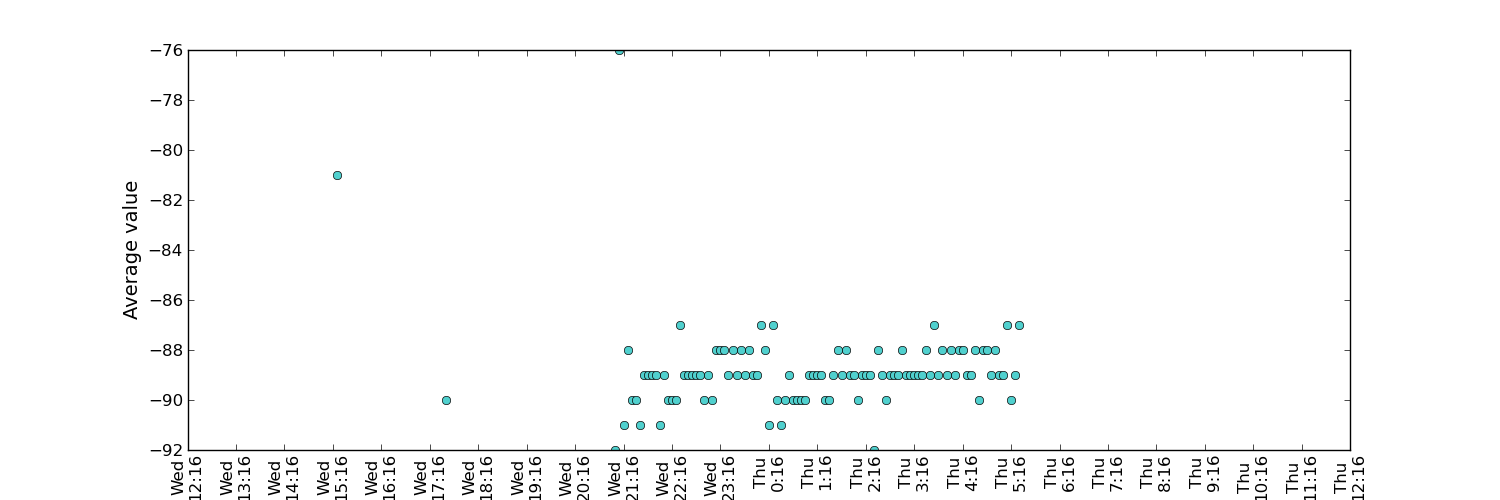
\includegraphics[width =\textwidth]{figures/combinations/user_6_sorted_1days_plot_3144_avg_sig.png}
\caption{Sample density of AP 3144}
\label{avg_6_2nd_day_3_A}
\end{figure}

\subsection{Running average signal strength}
\label{appendix_rn_avg}

This section contains the visualization for the running averages calculated for
$2$ (Fig.~\ref{user_1_AP1613_rn2avg_1d_A}), $5$
(Fig.~\ref{user_1_AP1613_rn2avg_1d_A}) and $10$
(Fig.~\ref{user_1_AP1613_rn2avg_1d_A}) minutes time bins for AP $1613$
identified in a time frame of one day (Fig.\ref{user_1_APs_1d_ap}).

\begin{figure}[!h]
\centering
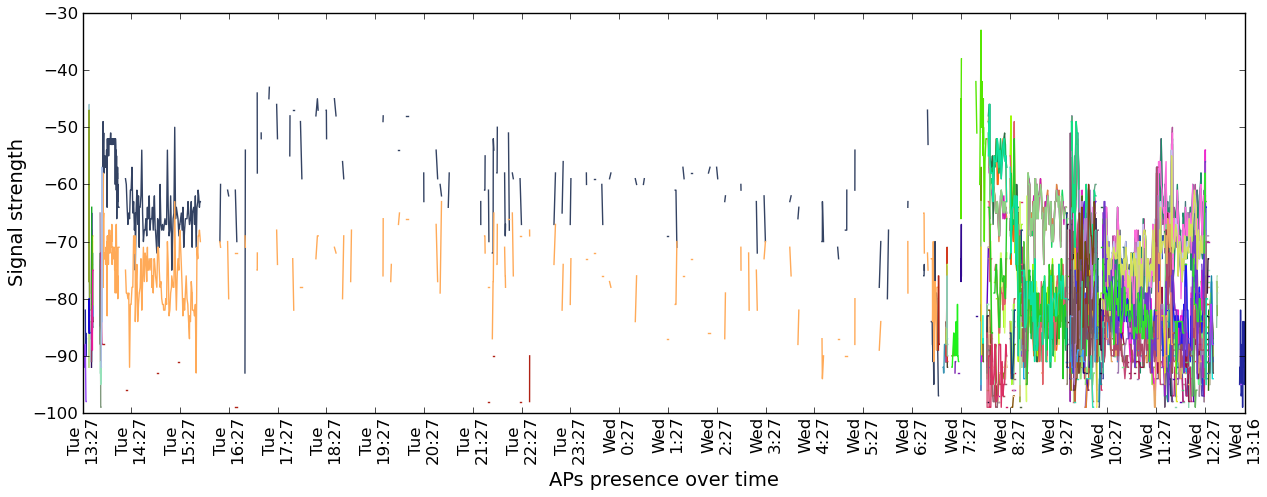
\includegraphics[width
=\textwidth]{figures/rn_avg/user_1_sorted_1days_plot.png}
\caption{Example of APs presence over time for userT}
\label{user_1_APs_1d_ap_A}
\end{figure}

\begin{figure}[!h]
\centering
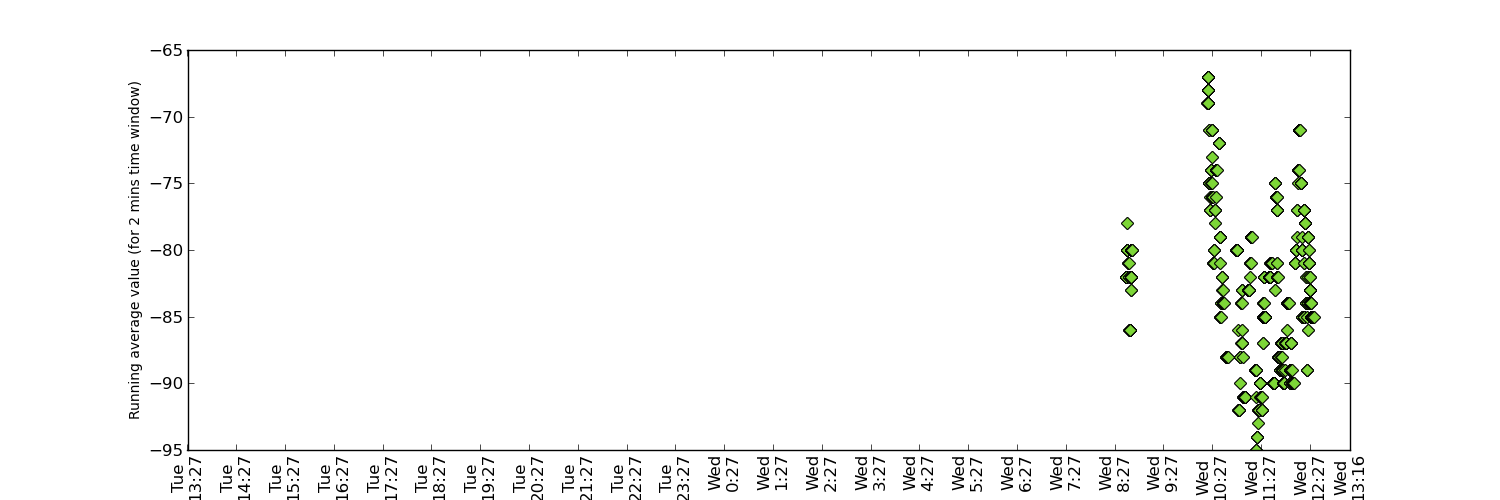
\includegraphics[width
=\textwidth]{figures/rn_avg/user_1_sorted_1days_plot_1613_rn_avg_sig_2.png}
\caption{Running average for AP 1613 for userT during 1 day (2 minute time
bins)}
\label{user_1_AP1613_rn2avg_1d_A}
\end{figure}

\begin{figure}[!h]
\centering
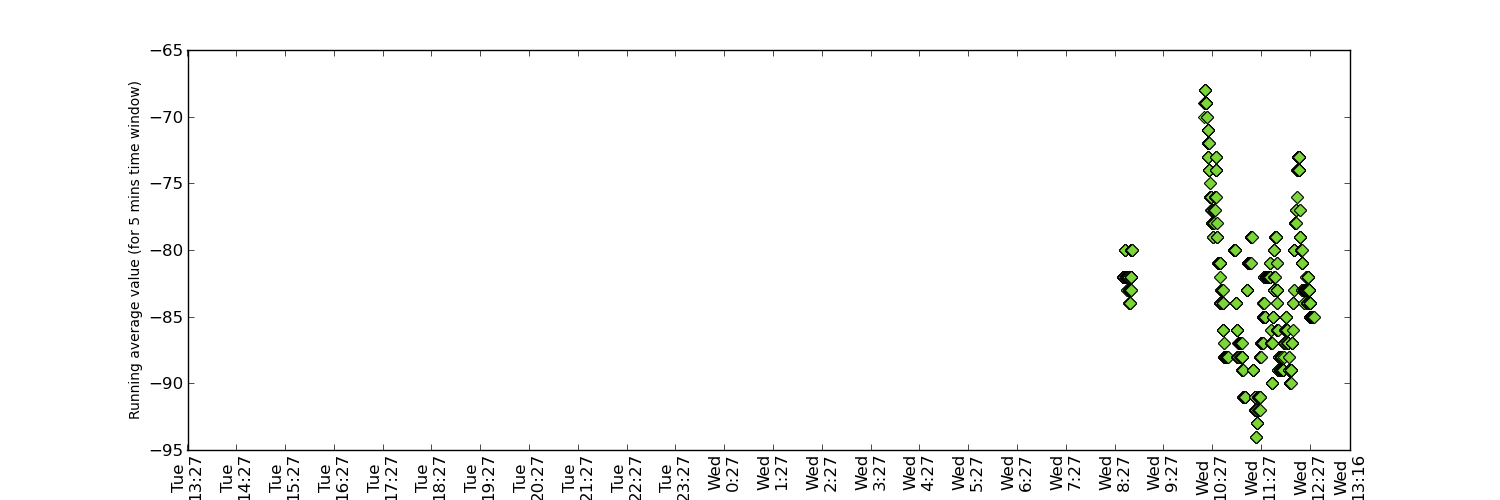
\includegraphics[width
=\textwidth]{figures/rn_avg/user_1_sorted_1days_plot_1613_rn_avg_sig_5.png}
\caption{Running average for AP 1613 for userT during 1 day (5 minute time
bins)}
\label{user_1_AP1613_rn5avg_1d_A}
\end{figure}

\begin{figure}[!h]
\centering
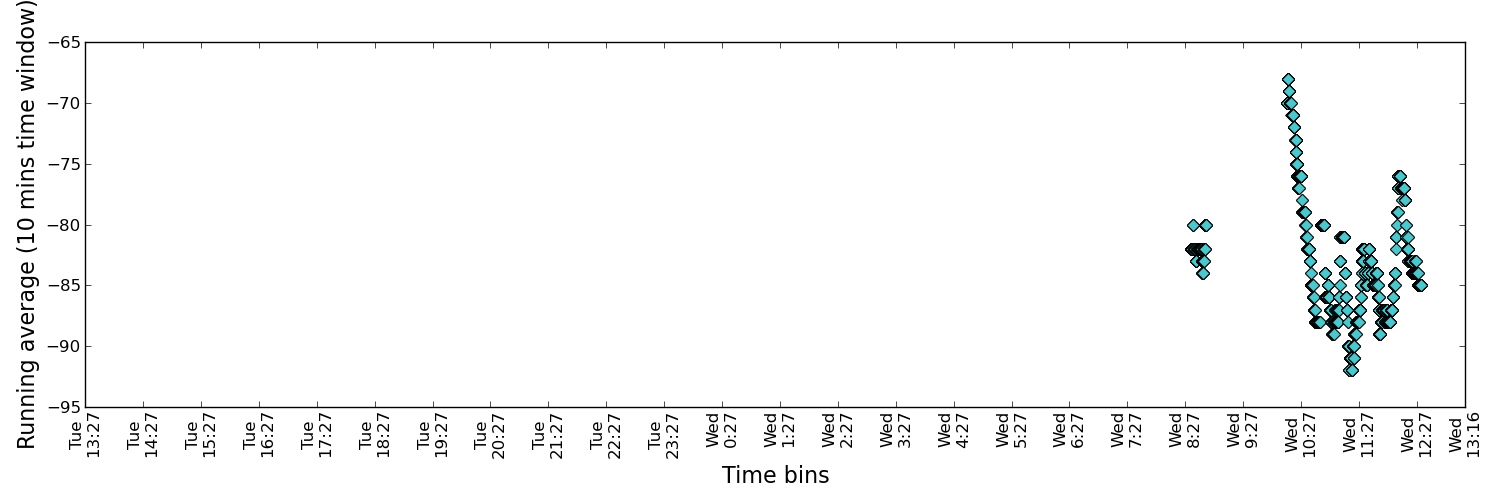
\includegraphics[width
=\textwidth]{figures/rn_avg/user_1_sorted_1days_plot_1613_rn_avg_sig_10.png}
\caption{Running average for AP 1613 for userT during 1 day (10 minute time
bins)}
\label{user_1_AP1613_rn10avg_1d_A}
\end{figure}

\subsection{Signal presence}
\label{appendix_pres}
This section contains the visualization for the presence of APs for a period of
$2$ days for an user from the SensibleDTU database
(Fig.~\ref{user_3_pres_2d_A}).The presence for APs is determined for $5$ minutes
time bins over the $2$ days.
Fig.~\ref{user_3_APs_2d_A} presents all the APs (and their signals) visualized
for the same $2$ days.

\begin{figure}[!h]
\centering
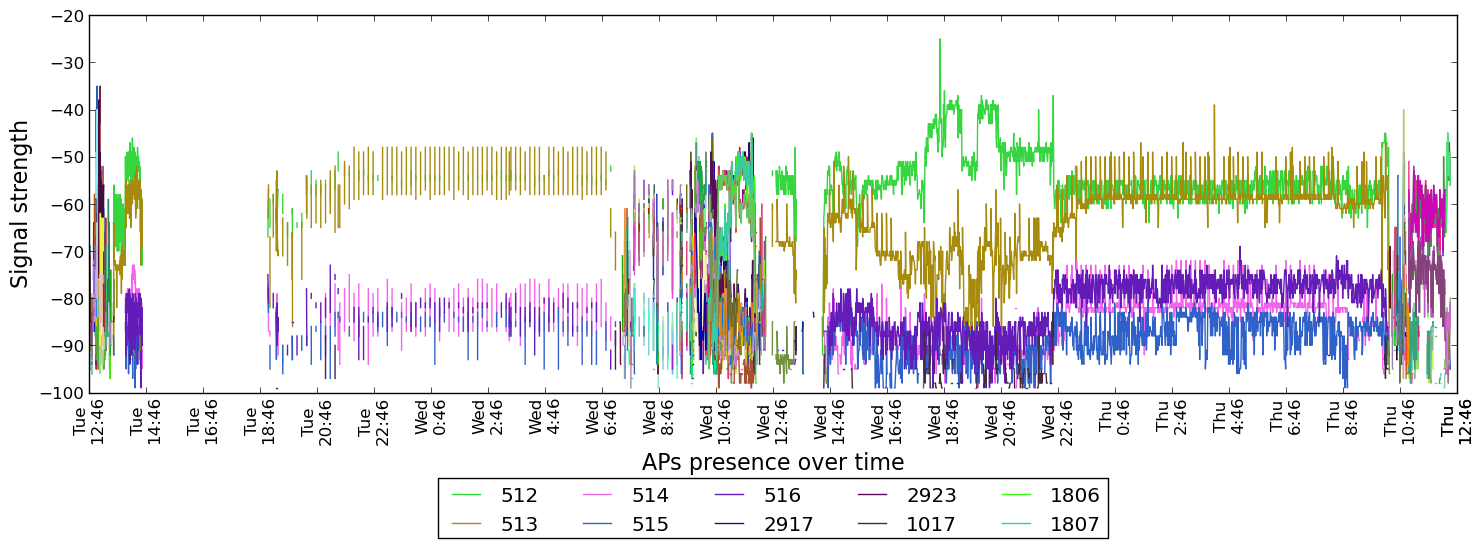
\includegraphics[width
=\textwidth]{figures/presence/user_3_sorted_2days_plot.png}
\caption{Scanned APs for an user throughout a duration of 2 days}
\label{user_3_APs_2d_A}
\end{figure}

\begin{figure}[!h]
\centering
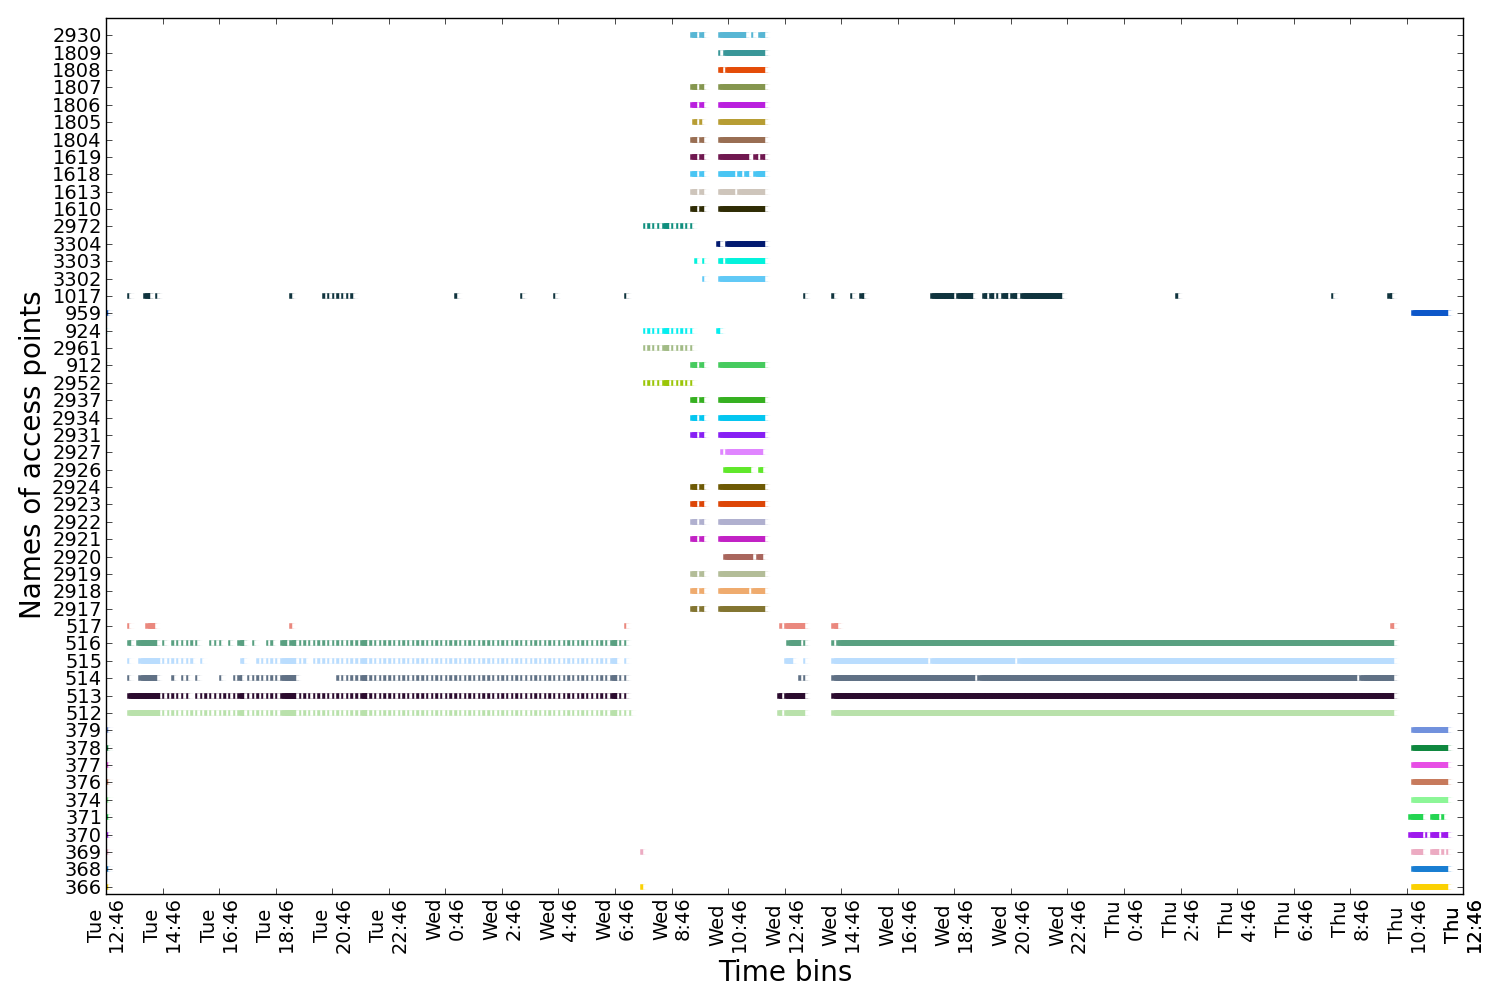
\includegraphics[width=1\textwidth]{figures/presence/user_3_sorted_2days_no_rssi_plot.png}
\caption{The most common 50 APs for an user during 2 days (presence
visualization calculated for 5 minutes time bins)}
\label{user_3_pres_2d_A}
\end{figure}

\subsection{Locations extracted using k-means}
\label{appendix_kmeans}
                                 %Appendix A
%-----------
% Backmatter
%-----------
\backmatter
\chaptermark{Bibliography}
\renewcommand{\sectionmark}[1]{\markright{#1}}
\sectionmark{Bibliography}
\addcontentsline{toc}{chapter}{Bibliography}        %Force addition of Bibliography to TOC
\bibliographystyle{alpha}                           %Use alpha codes for references
\bibliography{References}                           %Bibliography file called
\end{document}
% % % EOF % % %